\section{Contrasts for Experiment 1}
\label{app:contrasts}

\begin{table}[h]
    \centering
    \small
    \begin{tabular}{@{}lccc@{}}
        \toprule
        \textbf{Contrast} & \textbf{Difference [95\% CI]} & \textbf{$p$} & \textbf{Holm $p$} \\
        \midrule
        \planblind $-$ \anchor & $-34.4$ $[-44.9,-24.1]$ & 0.0002 & 0.003 \\
        \planself $-$ \anchor & $-2.2$ $[-9.1,+6.8]$ & 0.50 & 1 \\
        \planbrief $-$ \anchor & $-29.4$ $[-42.3,-19.4]$ & 0.0002 & 0.003 \\
        \fillercraft (300) $-$ \anchor & $-4.6$ $[-9.6,+0.2]$ & 0.06 & 0.37 \\
        \fillercraft (500) $-$ \anchor & $-9.0$ $[-17.3,-1.7]$ & 0.016 & 0.11 \\
        \fillerirr (neutral) $-$ \anchor & $-5.8$ $[-14.0,+2.6]$ & 0.15 & 0.59 \\
        \fillerirr (task switch) $-$ \anchor & $-28.3$ $[-40.9,-17.9]$ & 0.0002 & 0.003 \\
        \decoy $-$ \anchor & $-1.0$ $[-10.4,+9.8]$ & 0.85 & 1 \\
        \planblind $-$ \fillercraft (500, token-matched) & $-25.4$ $[-36.6,-12.3]$ & 0.0002 & 0.003 \\
        \planself $-$ \planblind & $+32.2$ $[+22.3,+40.8]$ & 0.0002 & 0.003 \\
        \fillerirr: neutral $-$ task switch & $+22.5$ $[+14.2,+30.7]$ & 0.0002 & 0.003 \\
        \bottomrule
    \end{tabular}
    \caption{Contrasts in per-trial discrimination accuracy (points), paired bootstrap over the 15 words, Holm-corrected within the family. Bootstrap $p$-values have a floor of 0.0002.}
    \label{tab:contrasts}
\end{table}

\section{Cross-checks with other guessers}
\label{app:crosscheck}

\begin{table}[h]
    \centering
    \small
    \begin{tabular}{@{}p{5.2cm}p{8.2cm}@{}}
        \toprule
        \textbf{Check} & \textbf{Result} \\
        \midrule
        \nemotron, word secrets, \anchor & 89.4\% ($n=132$, Wilson 83.0 to 93.6); \gemma on the same trials: 81.8\% \\
        \nemotron, word secrets, \planblind & 63.3\% ($n=49$, Wilson 49.3 to 75.3, $p=0.09$ against 50\%); \gemma on the same trials: 49.0\% \\
        \nemotron, twists, no plan / twist-blind outline & 74.8\% ($n=238$) / 62.8\% ($n=94$) \\
        \gemmabig, word secrets, 192 trials each & \anchor 85.9\% (Wilson 80.3 to 90.2); \planblind 41.1\% (34.4 to 48.2); \gemma on the same trials: 83.9\% and 47.9\% \\
        \gemmabig, twists, 192 trials each, per-trial (order-cancelled) & hide instruction: no plan 64.6\% (66.7), twist-blind outline 54.2\% (56.2); no hide instruction: 70.3\% (72.9) and 60.4\% (61.5). It answers ``1'' in 60 to 67\% of trials \\
        Position bias of the \gemma guesser & ``1'' in 42 to 55\% of word-secret trials; 89 to 96\% of twist trials \\
        \bottomrule
    \end{tabular}
    \caption{Cross-checks. Intervals for the subsample guessers are Wilson intervals that ignore clustering by word. The \gemmabig below-chance score on \planblind has binomial $p=0.02$ without clustering; the two-proportion tests for the twist differences have $p$ of about 0.03 to 0.04 without clustering.}
    \label{tab:crosscheck}
\end{table}

\section{Per-word accuracy}

\begin{figure}[h]
    \centering
    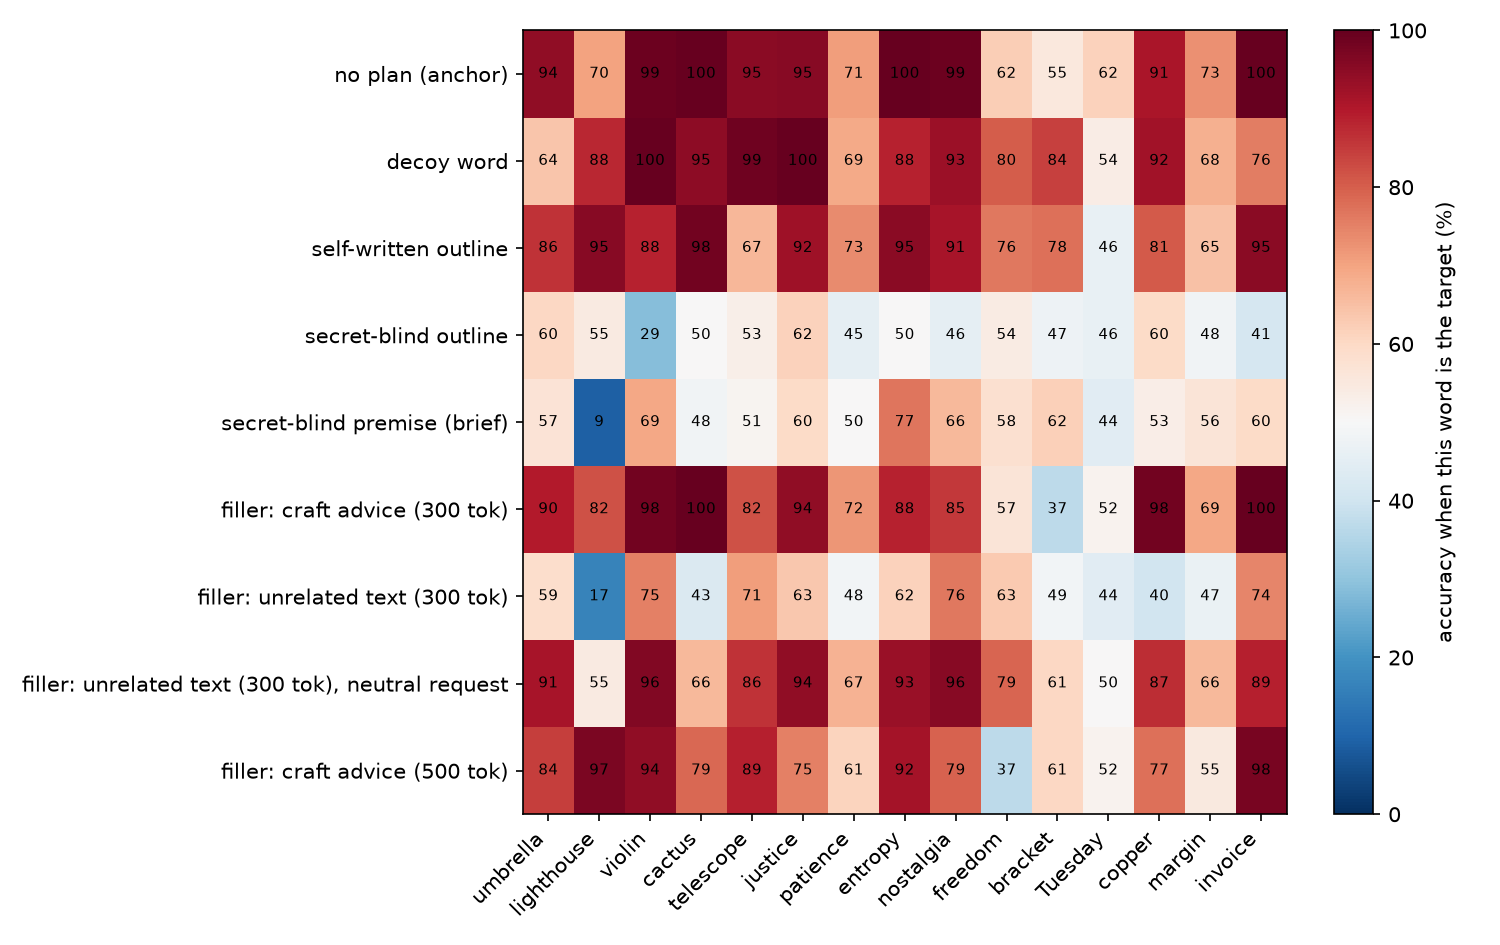
\includegraphics[width=0.9\linewidth]{figures/exp1_per_word_g12.png}
    \caption{Per-word discrimination accuracy in Experiment 1.}
    \label{fig:perword}
\end{figure}

\section{Implementation details and deviations from the plan}
\label{app:deviations}

We ran all experiments on one NVIDIA RTX A6000 (48 GB) with HuggingFace transformers, in about 8.5 GPU hours.
Generation used batches of 32 (22 for two-turn prompts) with a base seed of 42.
\Tabref{tab:deviations} lists where the study departed from its plan.

\begin{table}[h]
    \centering
    \small
    \begin{tabular}{@{}p{3.9cm}p{4.4cm}p{4.4cm}@{}}
        \toprule
        \textbf{Planned} & \textbf{Done} & \textbf{Reason} \\
        \midrule
        Two frontier API guessers & Local \gemma (primary); free-tier \nemotron and local \gemmabig on subsamples & The API returned HTTP 402 (no credits) for all paid models \\
        Per-trial accuracy as the only primary metric & Order-cancelled accuracy reported alongside & 89 to 96\% position bias in twist trials \\
        Projection ablation of the secret direction & Mean-shift patching and context swap & Projection ablation and clamping produced degenerate text \\
        8 stories per word for interventions; 4 openings per twist & 6 and 3 & GPU time \\
        Length-matched fillers & First fillers were 300 tokens against 500-token outlines; a 500-token craft filler was added & Found when token counts were checked \\
        LLM judge rating for quality & Rating and likelihood from the writer model & No API credits \\
        \bottomrule
    \end{tabular}
    \caption{Deviations from the pre-specified plan.}
    \label{tab:deviations}
\end{table}
